%!TEX program = xelatex
\documentclass{progartcn}
\usepackage{graphicx}
\usepackage[dvipsnames]{xcolor}
\usepackage{wrapfig}
\usepackage{enumerate}
\usepackage{appendix}
\usepackage{amsmath,mathrsfs,amsfonts}
\usepackage{booktabs}
\usepackage{tabularx}
\usepackage{colortbl}
\usepackage{multirow,makecell}
\usepackage{multicol}
\usepackage{ulem} % \uline
\usepackage{listings}
\usepackage{tikz}
\usepackage{tcolorbox}
\usepackage{fontawesome}
\usepackage{float}   %{H}
\usepackage{multicol}%分栏 %\begin{multicols}{2} %\end{multicols}
\usepackage{arydshln}
\setcounter{secnumdepth}{4}		%增加编号深度
\setcounter{tocdepth}{3}		%增加目录深度
\usepackage{hyperref}     %生成pdf书签
\hypersetup{hidelinks,
	colorlinks=true,
	allcolors=black,
	pdfstartview=Fit,
	breaklinks=true
}       %去掉目录的红色框框
\pagestyle{plain}%设置页码
\usepackage{fontspec}
\usepackage{enumitem} %调整有序列表的行距
\usepackage{makecell}
%\usepackage[colorlinks,linkcolor=blue]{hyperref}

\setCJKfamilyfont{hwzs}{STZHONGS.TTF}
\newcommand{\hwzs}{\CJKfamily{hwzs}}
\begin{document}

\sloppy % 解决中英文混排文字超出边界问题

\newpage

\thispagestyle{empty}
\begin{center}	
%	\parbox[t][1cm][c]{\textwidth}{\large
%		\begin{center} {\textbf{美团商业分析精英大赛}}\end{center} }
		
\includegraphics[width=2in]{2.jpg}\\
	\parbox[t][4cm][c]{\textwidth}{\Huge
		\begin{center} {\hwzs\textbf{专业课程实验报告}}\end{center} } %\heiti
		
	\parbox[t][1cm][t]{\textwidth}{
		\begin{center}  \end{center} }
	
%	\parbox[t][1cm][c]{\textwidth}{\Huge
%		\begin{center} {\hwzs{《程序设计综合课程设计》报告}}\end{center} }
	\parbox[t][10cm][b]{\textwidth}{
		\begin{center}
			\Large{
			\begin{tabular}{rl}
				% after \\: \hline or \cline{col1-col2} \cline{col3-col4} ...
				\textbf{课程名称}:& \underline{\;\;\;\;\;\;\;\;\;\;\;\;\;\;\;\;\;\;机器学习\;\;\;\;\;\;\;\;\;\;\;\;\;\;\;\;\;} \\
				\textbf{开课学期}:&{\underline{\;\;2021\;\;}至\underline{\;\;2022\;\;}学年\;\;第\underline{\;1\;}学期}\\
				\textbf{专\;\;\;\;\;\;\;业}:& \underline{\;\;\;\;\;\;\;\;\;智能科学与技术类\;\;\;\;\;\;\;\;\;\;\;\;}\\
				\textbf{年级班级}:&\underline{\;\;\;\;\;\;\;\;\;\;\;\;\;\;\;\;20级3班\;\;\;\;\;\;\;\;\;\;\;\;\;\;\;\;\;\;\;}\\
				\textbf{学生姓名}:& \underline{\;\;\;\;\;\;\;\;\;\;\;\;\;\;\;\;\;\;严中圣\;\;\;\;\;\;\;\;\;\;\;\;\;\;\;\;\;\;\;\;\;}\\
				\textbf{学生学号}:&\underline{\;\;\;\;\;\;\;\;\;\;\;\;222020335220177\;\;\;\;\;\;\;\;\;\;\;\;}\\
				\textbf{小\;\;组\;\;号}:&
				\underline{\;\;\;\;\;\;\;\;\;\;\;\;\;\;\;\;\;\;\;\;\;\;\;\;1\;\;\;\;\;\;\;\;\;\;\;\;\;\;\;\;\;\;\;\;\;\;\;\;}\\
				\textbf{实验教师}:& \underline{\;\;\;\;\;\;\;\;\;\;\;\;\;\;\;\;\;\;\;\;\;褚金\;\;\;\;\;\;\;\;\;\;\;\;\;\;\;\;\;\;\;\;\;}\\
			\end{tabular}}
		\end{center} }
	
	\parbox[t][4cm][b]{\textwidth}{
		\begin{center} {\large{\textsf 人工智能学院}} \end{center} }
\end{center}


\clearpage
%=============================================================================================
%\maketitle
\thispagestyle{empty}
%\tableofcontents  %目录
\newpage

\parbox[t][0.5cm][b]{\textwidth}{\begin{center} {\Large\textbf{\textsf 《机器学习》实验课报告书}} \end{center} }

\parbox[t][2cm][b]{\textwidth}{
%	\begin{center}
		\large{
			\begin{tabular}{rlrl}
				% after \\: \hline or \cline{col1-col2} \cline{col3-col4} ...
				\textbf{实验编号}:& \underline{\;\;\;\;\;\;\;\;\;\;\;\;\;\;\;1\;\;\;\;\;\;\;\;\;\;\;\;\;\;\;\;\;\;\;\;\;}&
				\textbf{实验名称}:&\underline{\;\;\;BP神经网络用于分类\;\;\;}\\
					
				\textbf{姓\;\;\;\;\;\;\;名}:&\underline{\;\;\;\;\;\;\;\;\;\;\;\;\;严中圣\;\;\;\;\;\;\;\;\;\;\;\;\;\;}&
				\textbf{学\;\;\;\;\;\;\;号}:&\underline{\;\;\;\;\;\;\;222020335220177\;\;\;\;\;\;\;}\\
				
				\textbf{日\;\;\;\;\;\;\;期}:&\underline{\;\;\;\;\;\;2021年 11 月 6 日\;\;\;\;\;}&
				\textbf{教师打分}:&\underline{\;\;\;\;\;\;\;\;\;\;\;\;\;\;\;\;\;\;\;\;\;\;\;\;\;\;\;\;\;\;\;\;\;\;\;\;\;\;\;\;}\\
		\end{tabular}}
%\end{center} 
}


\section{实验摘要}

本次实验要求利用BP神经网络实现多分类任务。数据集选用\href{http://archive.ics.uci.edu/ml/datasets/Statlog+\%28Vehicle+Silhouettes\%29}{Statlog (Vehicle Silhouettes) Data Set} ,共计18个特征,4个类别属性,846条数据。我们建立了四层神经网络进行分类任务,其中包含两个隐藏层,输出层采用sigmoid函数,在原始数据集上达到了72.352941\%的准确率。为了进一步提高准确率,我们首先对数据集进行了预处理,由于发现特征间存在很强的复共线性,故利用因子分析提取出5个公因子,再利用Z-score进行数据标准化;同时引入了学习率逐步衰减机制,使训练收敛更为精准,最后经训练测试集可达90\%的准确率,良好的完成了分类任务。

\section{程序流程框图}

\begin{figure}[H]
	\centering
	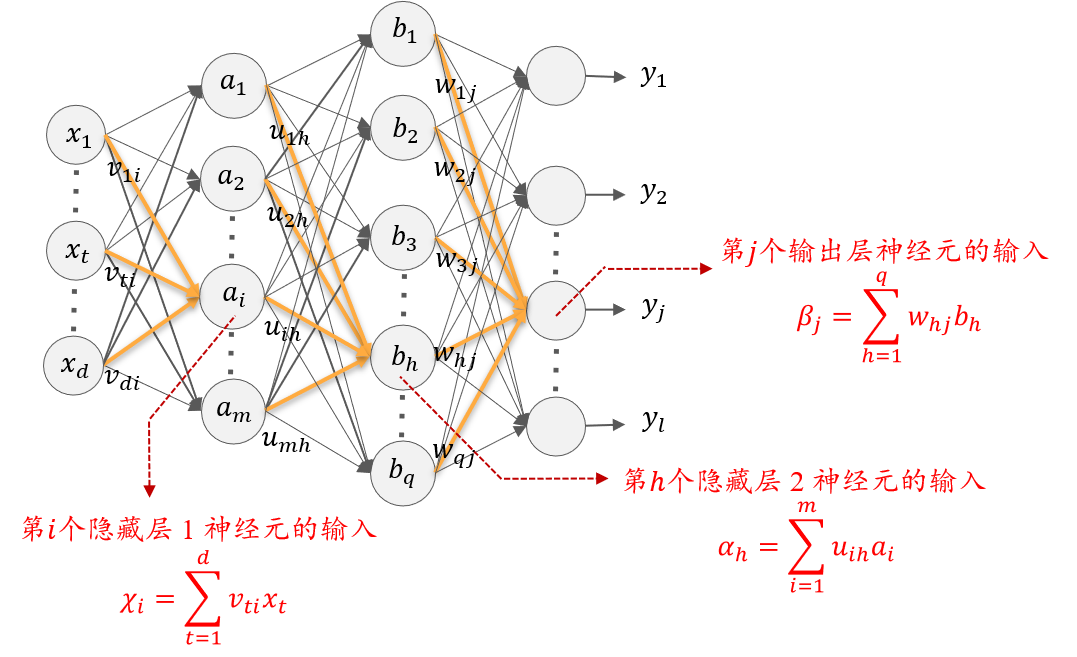
\includegraphics[width=0.8\textwidth]{图片1.png}
	\caption{\centering  网络结构设计图}
\end{figure}
\begin{equation}
	\begin{aligned}
		a_m &= f(\chi_i-e_i) \\
		b_h &= f(\alpha_h - \gamma_h) \\
		y_j &= f(\beta_j - \theta_j) \\
	\end{aligned}
\end{equation}
如图1所示,网络结构设计为四层网络层,包括一个输入层,一个输出层和两个隐藏层。数据输入后,通过误差逆传播(BP)算法对其中的权值及偏置进行不断更新。

\section{实验原理}
\subsection{神经元模型}
神经网络(Neural Network)是由具有适应性的简单单元组成的广泛并行互连的网络,它的组织能够模拟生物神经系统对真实世界物体所作出的交互反应。神经网络中最基本的成分是神经元模型,即上述定义中的"简单单元"在生物神经网络中每个神经元与其他神经元相连,当它"兴奋"时,就会向相连的神经元发送化学物质,从而改变这些神经元内的电位;如果某神经元的电位超过了一个"阔值" (threshold)那么它就会被激活,即"兴奋"起来,向其他神经元发送化学物质.

\begin{figure}[H]
	\centering
	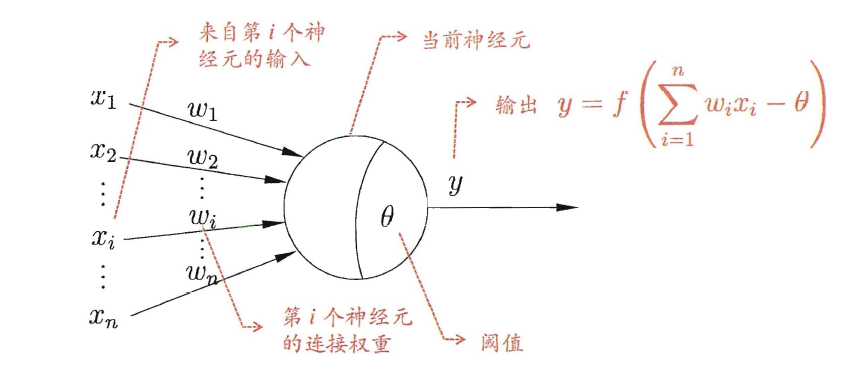
\includegraphics[width=0.7\linewidth]{screenshot001}
	\caption{\centering M-P神经元模型}
	\label{fig:screenshot001}
\end{figure}
\subsection{误差逆传播算法}
对于我们所设计的如图一所示的网络结构,我们设置隐层神经元为ReLU函数,输出层采用Sigmoid函数
\begin{equation}
	\begin{aligned}
		f_1&=ReLU(x)=\left\{\begin{aligned}
			x \quad x>0 \\
			0 \quad x\leq 0 \\
		\end{aligned}\right. \\
		f_2&=Sigmoid(x)=\frac{1}{1+e^{-x}}\\
	\end{aligned}
\end{equation}
此外设置损失函数为
\begin{equation}
	E_k=\frac{1}{2} \sum_{j=1}^{l}(\hat{y_j^k-y_j^k})^2
\end{equation}
BP 是一个迭代学习算法,在迭代的每一轮中采用广义的感知机学习规则对参数进行更新估计,则任意参数$v$的更新估计式为
\begin{equation}
	v \leftarrow v+\Delta v
\end{equation}
于是基于梯度下降策略,以目标的负梯度方向对参数进行调整,对式(3)的误差$E_k$,给定学习率$\eta$,有:
\begin{equation}
	\begin{aligned}
		\Delta w_{hj}=-\eta \frac{\partial E_k}{\partial w_{hj}} \\
	\end{aligned}
\end{equation}
根据链式法则:
\begin{equation}
	\frac{\partial E_k}{\partial w_{hj}}=\frac{\partial E_k}{\partial \hat{y_j}^k}\frac{\partial \hat{y_j}^k}{\partial \beta_j}\frac{\partial \beta_j}{\partial w_{hj}}
\end{equation}
根据$\beta_j$的定义,显然有
\begin{equation}
	\frac{\partial \beta_j}{\partial w_{hj}}=b_h
\end{equation}
此外Sigmoid函数有一个很好的性质
\begin{equation}
	f'(x)=f(x)(1-f(x))
\end{equation}
于是设
\begin{equation}
	g_j=-\frac{\partial E_k}{\partial \hat{y_j}^k}\frac{\partial \hat{y_j}^k}{\partial \beta_j}=\hat{y_j}^k(1-\hat{y_j}^k)(y_j^k-\hat{y_j}^k)
\end{equation}
所以$w_{hj}$的更新公式为
\begin{equation}
	\Delta w_{hj}=\eta g_jb_h
\end{equation}
同理可得:
输出层偏置$\theta_j$的更新公式为:
\begin{equation}
	\Delta \theta_j=-\eta g_j
\end{equation}
隐藏层2的权重及偏置更新公式为:
\begin{equation}
	\begin{aligned}
		\Delta u_{ih}&=-\eta \frac{\partial E_k}{\partial u_{ih}} \\		
		&=-\eta \sum_{j=1}^{l}-g_jw_{hj}b_h(1-b_h)a_i \\
		&=\sum_{j=1}^{l}\eta g_jw_{hj}b_h(1-b_h)a_i \\
		\Delta \gamma_h &=-\eta \frac{\partial E_k}{\partial \gamma_h} \\
		&=-\sum_{j=1}^{l}\eta g_jw_{hj}b_h(1-b_h) \\
	\end{aligned}
\end{equation}
隐藏层1的权重及偏置更新公式为:
\begin{equation}
	\begin{aligned}
		\Delta v_{ti}&=-\eta \frac{\partial E_k}{\partial v_{ti}} \\
		&=-\sum_{j=1}^{l}\sum_{h=1}^{q}\eta g_jw_{hj}b_h(1-b_h)u_{ih}a_i(1-a_i)x_t \\
		\Delta e_i &=-\eta \frac{\partial E_k}{\partial e_i} \\
		&=\sum_{j=1}^{l}\sum_{h=1}^{q}\eta g_jw_{hj}b_h(1-b_h)u_{ih}a_i(1-a_i)
	\end{aligned}
\end{equation}

\section{数据预处理及实验结果}

\subsection{数据预处理}

针对所给数据集,我们首先分析了数据之间的相关性,得出相关系数热力图如附录1所示,可以发现许多特征之间仅仅是线性相关性便已经达到接近于1的相关性,这说明数据间存在很强的复共线性,极容易发生过拟合,故我们对数据进行因子分析提取主要特征。

首先对数据进行KMO检验和Bartlett球形检验,结果KMO测度为0.8070,$p_{value}=0.00336$,这进一步说明了变量间的相关性很强,适合作因子分析。对数据进行因子分析后,共提取5个公因子,方差解释率到达91\%,具体数据见附件Factor\_data.xlsx,代码见附录2。

其次又发现数据间由于量纲等原因造成了巨大差异,故采用Z-score标准化对数据进行处理
\begin{equation}
	x^*=\frac{x-\mu}{\sigma}
\end{equation}

\subsection{网络训练过程及实验结果}
起初我们固定学习率进行训练时,若学习率过大尽管可以快速趋于极大值,但是最后会出现极大的波动,导致无法收敛,若学习率过小又会导致收敛过慢,训练时间太长。故为了更好的达到收敛效果,我们引入了学习率衰减机制,利用指数减缓的方式进行调整
\begin{equation}
	\eta =0.95^{epoch\_num}*\eta_0
\end{equation}
下面对网络进行训练,训练结果在训练集上准确率可达90.107379\%,在测试集数据上准确率达到了88.584475\%,可见如期比较良好地完成了分类任务。


\section{实验总结}
%在训练会出现以下几个问题
%sigmoid函数溢出,展平再reshape
%收敛过快

本次实验手写了一个含两个隐藏层的BP神经网络实现了多分类任务,在编码的过程中加深了对算法的理解,同时也掌握了许多算法优化的方法,也很好地锻炼的数学推导和编写程序的能力,也进一步地感受到了神经网络的强大之处。神经网络算法在当前深度学习火热的大环境下,广泛运用于图像处理、自然语言处理、控制算法等多个领域,一再验证了其效果的强大。这也更激励着我对神经网络和深度学习领域进一步的探索,期待未来能够为此领域做出自己的贡献。

\section{参考文献}
\begin{enumerate}[itemsep=0.01pt]
	\item[] [1] 周志华. 机器学习[M]. 清华大学出版社, 2016.
	\item[] [2] Smith L N. Cyclical learning rates for training neural networks[C]//2017 IEEE winter conference on applications of computer vision (WACV). IEEE, 2017: 464-472.
	\item[] [3] https://zhuanlan.zhihu.com/p/285601835
	\item[] [4] https://blog.csdn.net/han\_xiaoyang/article/details/50521064
\end{enumerate}




=======================================================================\\
\textbf{三线表: }
\begin{table}[H]
	\renewcommand{\arraystretch}{1.0}
	\centering
	\caption{\centering “添加好友”页界面各控件属性设置}
	\begin{tabular}{lll}
		\toprule[1.5pt]
	名称&类型&属性设置\\
		\midrule[1pt]
		newGroupComboBox  & QComboBox & 默认\\
		newIDLineEdit      & QLineEdit   & 默认\\
		FriendsTableView     & QTableView  & \makecell[l]{horizontalHeaderVisibe:勾选\\ horizontalHeaderDefaultSectionSize:120\\ horizontalHeaderMinimumSectionSize:25\\ horizionHeaderStretchLastSection:勾选\\ verticalHeaderVisible:取消勾选}
		\\
		\bottomrule[1.5pt]
	\end{tabular}
\end{table}

\textbf{有序列表:}
\begin{enumerate}[itemsep=0.01pt]
	\item[(1)] 能够实现QQ登录系统并具有独立的登录界面;
	\item[(2)] 能够实现用户通过口令登录,且密码采用MD5加密算法封装验证;
	\item[(3)] 能够实现QQ好友管理系统并具有独立的系统界面;
	\item[(4)] 能够实现通过鼠标触发事件进行软件操作;
\end{enumerate}

\textbf{代码块:}
\begin{lstlisting}[language=c++]
QString LoginDialog::strToMd5(QString str)
{
	QString strMd5;
	QByteArray qba;
	qba=QCryptographicHash::hash(str.toLatin1(),QCryptographicHash::Md5);//调用QCryptographicHash类中生成密码散列的方法,生成二进制或文本数据的加密散列值
	strMd5.append(qba.toHex());
	return strMd5;
}	
\end{lstlisting}



\newpage
\begin{center}
	\Large{\textbf{\heiti 附录}}
\end{center}

\appendix
% \renewcommand{\appendixname}{Appendix~\Alph{section}}
\section{附录 1 -- 原始数据相关系数热力图 }
\begin{figure}[H]
	\centering
	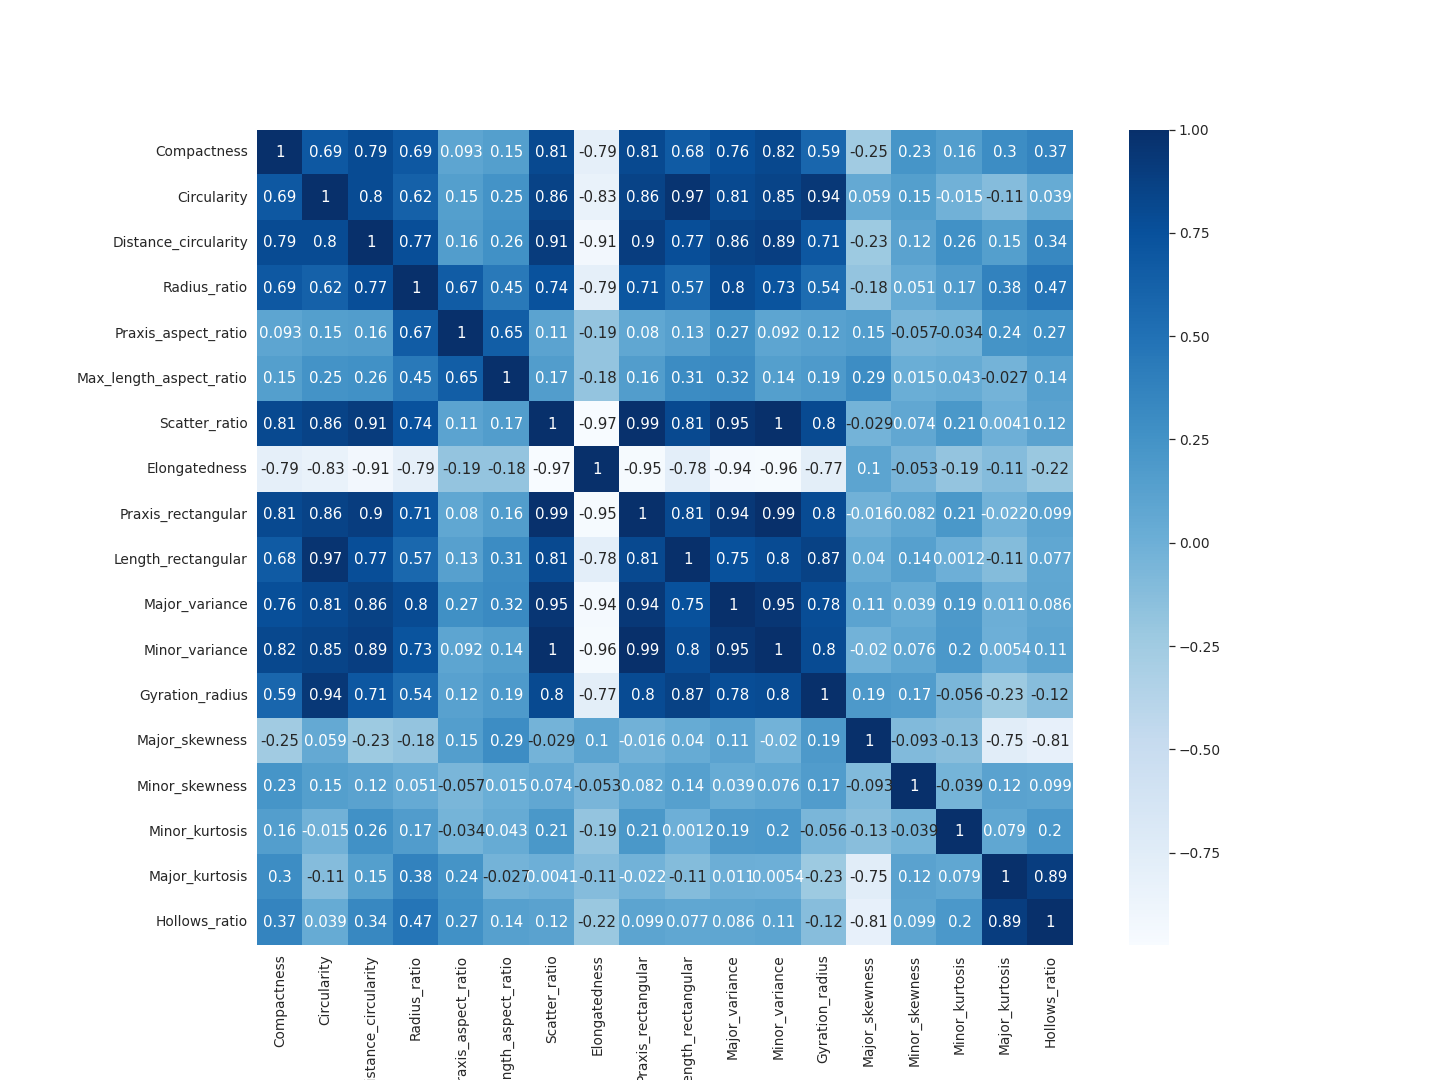
\includegraphics[width=0.8\linewidth]{corr.png}
	\caption{\centering 相关系数热力图}
	\label{fig:screenshot001}
\end{figure}

\section{附录 2 -- 因子分析代码 }
\lstinputlisting[language=Python]{./code/1.txt}

\section{附录 3 -- BP神经网络训练代码 }
\lstinputlisting[language=Python]{./code/2.txt}
\end{document}